\documentclass[tikz,border=8pt]{standalone}
% Shared look for every TikZ diagram. Load with \input{../../tools/tikz-style.tex}
\usepackage[T1]{fontenc}
\usepackage{lmodern}
\renewcommand{\sfdefault}{lmr}  % diagrams use the same serif as the text
\usetikzlibrary{arrows.meta, positioning, shapes.geometric, calc, fit, backgrounds}
\definecolor{cblue}{HTML}{4C78A8}
\definecolor{corange}{HTML}{F58518}
\definecolor{cgreen}{HTML}{54A24B}
\definecolor{cred}{HTML}{E45756}
\definecolor{cpurple}{HTML}{B279A2}
\definecolor{cgrey}{HTML}{6B6B6B}
\tikzset{
  every picture/.style={font=\sffamily, line width=1.2pt},
  box/.style={draw=#1, fill=#1!12, rounded corners=4pt, align=center, inner sep=7pt, minimum height=1.1cm},
  box/.default=cgrey,
  arrow/.style={-{Stealth[length=3mm]}, draw=cgrey, line width=1.4pt},
  title/.style={font=\sffamily\bfseries\Large},
  note/.style={font=\sffamily\small, text=cgrey, align=center},
}
\AtBeginDocument{\hyphenpenalty=10000 \exhyphenpenalty=10000}

\begin{document}
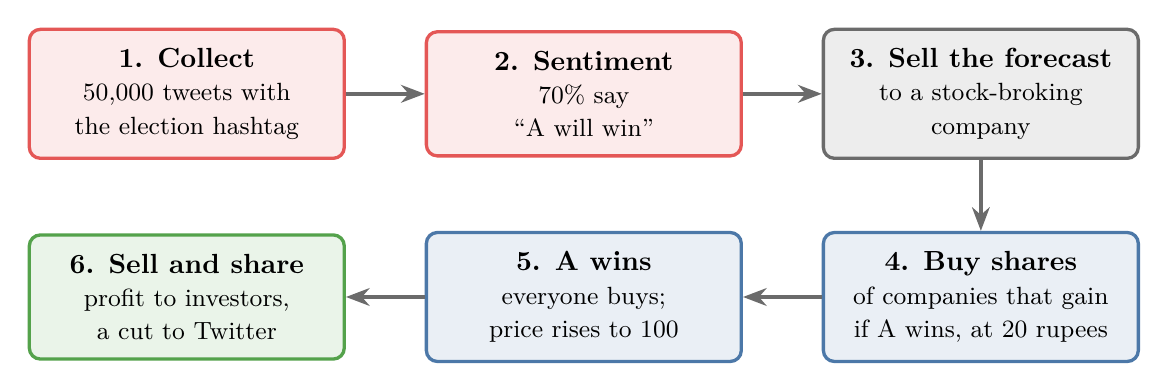
\begin{tikzpicture}[node distance=0.9cm and 1.0cm]
  \tikzset{step/.style={box=#1, minimum width=4.0cm, minimum height=1.5cm}}
  \node[step=cred] (a) {\textbf{1. Collect}\\{\small 50,000 tweets with}\\{\small the election hashtag}};
  \node[step=cred, right=of a] (b) {\textbf{2. Sentiment}\\{\small 70\% say}\\{\small ``A will win''}};
  \node[step=cgrey, right=of b] (c) {\textbf{3. Sell the forecast}\\{\small to a stock-broking}\\{\small company}};
  \node[step=cblue, below=of c] (d) {\textbf{4. Buy shares}\\{\small of companies that gain}\\{\small if A wins, at 20 rupees}};
  \node[step=cblue, left=of d] (e) {\textbf{5. A wins}\\{\small everyone buys;}\\{\small price rises to 100}};
  \node[step=cgreen, left=of e] (f) {\textbf{6. Sell and share}\\{\small profit to investors,}\\{\small a cut to Twitter}};
  \draw[arrow] (a) -- (b); \draw[arrow] (b) -- (c); \draw[arrow] (c) -- (d);
  \draw[arrow] (d) -- (e); \draw[arrow] (e) -- (f);
\end{tikzpicture}
\end{document}
